% Preamble
% ---
\documentclass{article}

% Packages
% ---
\usepackage{amsmath} % Advanced math typesetting
\usepackage[utf8]{inputenc} % Unicode support (Umlauts etc.)
\usepackage[ngerman]{babel} % Change hyphenation rules
\usepackage{hyperref} % Add a link to your document
\usepackage{graphicx} % Add pictures to your document
\usepackage{listings} % Source code formatting and highlighting
\usepackage{booktabs}

\renewcommand{\figurename}{Figure}
%\usepackage[labelsep=endash]{caption}

\usepackage{xcolor}
\lstset { %
    language=C++,
    backgroundcolor=\color{black!5}, % set backgroundcolor
    basicstyle=\footnotesize,% basic font setting
}



\title{%
	MA226 : Monte-Carlo Simulation\\
	 Generating Numbers from Discrete Distributions and Mixture Distributions\\
	 \large Assignment 7}

\date{20-03-2017}

\author{%
	Turkhade Hrushikesh Pramod\\
	150123044	}	

\begin{document}

	\maketitle
	\pagenumbering{gobble}
	
	\newpage
	\pagenumbering{arabic}
	
	\section{Problem 1}
	\paragraph{}
		Here we have to generate numbers from Geometric Distribution.
		
	\subsection{Source code of the solution}
		\lstinputlisting[language=R,firstline=1]{code/que1.r}
	
	\subsection{Plot}
			\begin{figure}
  				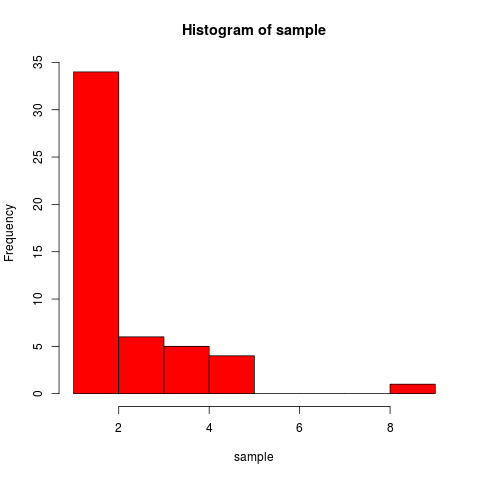
\includegraphics[width=\linewidth]{pic/que1.png}
 			 	\caption{Histogram of Generated Geometric Distribution}
  			\label{fig:hist1}
		\end{figure}
	\clearpage		
	
	\section{Problem 2}
		In this problem, we have to generate numbers from Poisson Distribution.
		
	\subsection{Source code of the solution}
		\lstinputlisting[language=R,firstline=1]{code/que2.r}
		
	\subsection{Plot}
		
		\begin{figure}[!ht]
  			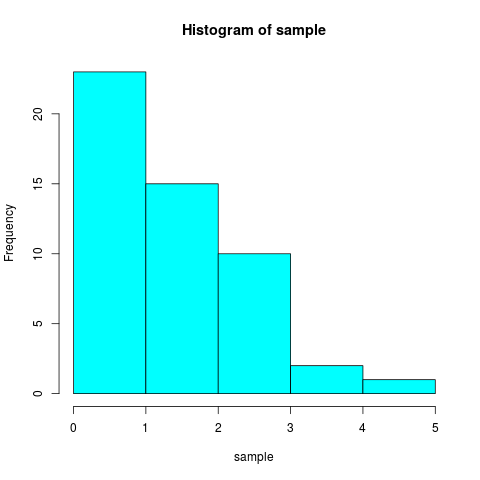
\includegraphics[width=\linewidth]{pic/que2.png}
 			 \caption{PDF of the Generated Poisson Distribution}
  			\label{fig:hist1}
		\end{figure}
		
		\begin{figure}[!ht]
  			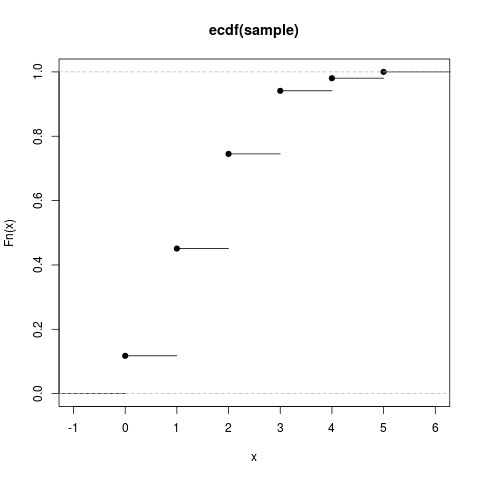
\includegraphics[width=\linewidth]{pic/que2_cdf.png}
 			 \caption{CDF of Generated Poisson Distribution}
  			\label{fig:hist1}
		\end{figure}
		
		\clearpage
		

			
	\section{Problem 3}
		\paragraph{}
			In this problem, we have to generate a distribution which is a mixture distribution. The mixture distribution conssists of two weibull distritution.
			
			
		\subsection{Source code of the solution}
			\lstinputlisting[language=r,firstline=1]{code/que3.r}
			
		\subsection{Plot of the points}
			\begin{figure}[ht]
  				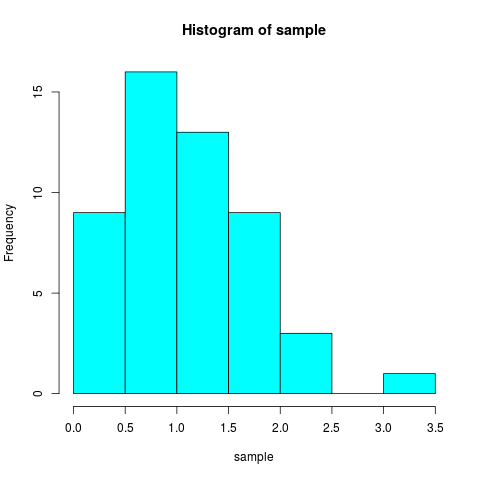
\includegraphics[width=\linewidth]{pic/que3.png}
 			 	\caption{2D plot for ($u_{i-1},u_i$) , seed=7}
  			\label{fig:hist1}
		\end{figure}
		.
	

\end{document}